% 原卷第23题三棱锥；D 按题干为 AC 上交点，原图标签按可见记号保留为 D'。
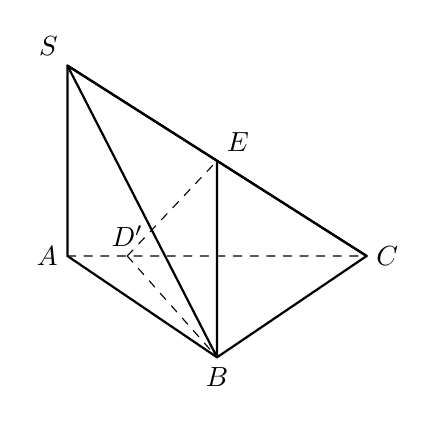
\begin{tikzpicture}[x=0.95cm,y=0.78cm,line cap=round,line join=round]
  \coordinate (A) at (-1.6,0);
  \coordinate (C) at (2.4,0);
  \coordinate (B) at (0.4,-1.65);
  \coordinate (S) at (-1.6,3.1);
  \coordinate (D) at (-0.8,0);
  \coordinate (E) at (0.4,1.55);
  \draw[thick] (A)--(S)--(C)--(B)--cycle;
  \draw[thick] (S)--(B) (S)--(E) (E)--(C) (E)--(B);
  \draw[dashed] (A)--(C) (D)--(B) (D)--(E);
  \node[above left] at (S) {$S$};
  \node[left] at (A) {$A$};
  \node[below] at (B) {$B$};
  \node[right] at (C) {$C$};
  \node[above] at (D) {$D'$};
  \node[above right] at (E) {$E$};
\end{tikzpicture}
